43. $|y|=|x-1|\Leftrightarrow \left[\begin{array}{l}y=x-1,\\ y=1-x.\end{array}\right.$
$$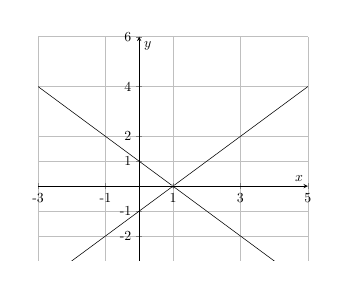
\begin{tikzpicture}[scale=0.5]
\begin{axis}[
    axis lines = middle,
    grid=major,
    legend pos={south west},
    xlabel = {$x$},
    ylabel = {$y$},
    ymin=-3,
    ymax=6,
    xtick={-3,-1,1,3,5},
    xticklabels={-3,-1,1,3,5},
    ytick={ 6, 2,-6, -2,1,-1,4,-4},
    yticklabels={ 6, 2,-6, -2,1,-1,4,-4}           ]
	\addplot[domain=-3:5, samples=100, color=black] {abs(x-1)};
\addplot[domain=-3:5, samples=100, color=black] {-abs(x-1)};
%\addplot[domain=-3.1:2.5, samples=100, color=red] {70*abs(1-2*abs(abs(x)-2))-10*x^2+10*x-70};
	%\addlegendentry{$\text{Рис. 1}$};
\end{axis}
\end{tikzpicture}$$
